% Created by tikzDevice version 0.12.3.1 on 2021-01-15 15:47:44
% !TEX encoding = UTF-8 Unicode
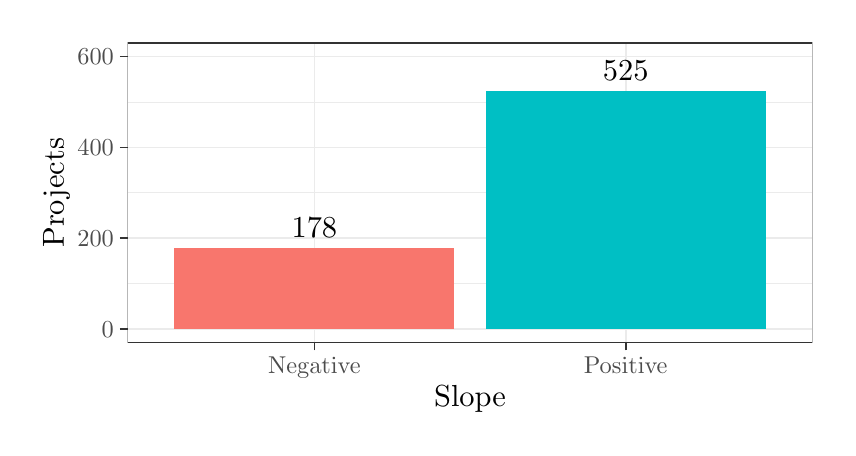
\begin{tikzpicture}[x=1pt,y=1pt]
\definecolor{fillColor}{RGB}{255,255,255}
\path[use as bounding box,fill=fillColor,fill opacity=0.00] (0,0) rectangle (289.08,144.54);
\begin{scope}
\path[clip] (  0.00,  0.00) rectangle (289.08,144.54);
\definecolor{drawColor}{RGB}{255,255,255}
\definecolor{fillColor}{RGB}{255,255,255}

\path[draw=drawColor,line width= 0.6pt,line join=round,line cap=round,fill=fillColor] (  0.00,  0.00) rectangle (289.08,144.54);
\end{scope}
\begin{scope}
\path[clip] ( 36.11, 30.69) rectangle (283.58,139.04);
\definecolor{fillColor}{RGB}{255,255,255}

\path[fill=fillColor] ( 36.11, 30.69) rectangle (283.58,139.04);
\definecolor{drawColor}{gray}{0.92}

\path[draw=drawColor,line width= 0.3pt,line join=round] ( 36.11, 52.03) --
	(283.58, 52.03);

\path[draw=drawColor,line width= 0.3pt,line join=round] ( 36.11, 84.86) --
	(283.58, 84.86);

\path[draw=drawColor,line width= 0.3pt,line join=round] ( 36.11,117.70) --
	(283.58,117.70);

\path[draw=drawColor,line width= 0.6pt,line join=round] ( 36.11, 35.61) --
	(283.58, 35.61);

\path[draw=drawColor,line width= 0.6pt,line join=round] ( 36.11, 68.45) --
	(283.58, 68.45);

\path[draw=drawColor,line width= 0.6pt,line join=round] ( 36.11,101.28) --
	(283.58,101.28);

\path[draw=drawColor,line width= 0.6pt,line join=round] ( 36.11,134.11) --
	(283.58,134.11);

\path[draw=drawColor,line width= 0.6pt,line join=round] (103.60, 30.69) --
	(103.60,139.04);

\path[draw=drawColor,line width= 0.6pt,line join=round] (216.09, 30.69) --
	(216.09,139.04);
\definecolor{fillColor}{RGB}{248,118,109}

\path[fill=fillColor] ( 52.98, 35.61) rectangle (154.22, 64.83);
\definecolor{fillColor}{RGB}{0,191,196}

\path[fill=fillColor] (165.47, 35.61) rectangle (266.71,121.80);
\definecolor{drawColor}{RGB}{0,0,0}

\node[text=drawColor,anchor=base,inner sep=0pt, outer sep=0pt, scale=  1.10] at (103.60, 68.64) {178};

\node[text=drawColor,anchor=base,inner sep=0pt, outer sep=0pt, scale=  1.10] at (216.09,125.60) {525};
\definecolor{drawColor}{gray}{0.20}

\path[draw=drawColor,line width= 0.6pt,line join=round,line cap=round] ( 36.11, 30.69) rectangle (283.58,139.04);
\end{scope}
\begin{scope}
\path[clip] (  0.00,  0.00) rectangle (289.08,144.54);
\definecolor{drawColor}{gray}{0.30}

\node[text=drawColor,anchor=base east,inner sep=0pt, outer sep=0pt, scale=  0.88] at ( 31.16, 32.58) {0};

\node[text=drawColor,anchor=base east,inner sep=0pt, outer sep=0pt, scale=  0.88] at ( 31.16, 65.42) {200};

\node[text=drawColor,anchor=base east,inner sep=0pt, outer sep=0pt, scale=  0.88] at ( 31.16, 98.25) {400};

\node[text=drawColor,anchor=base east,inner sep=0pt, outer sep=0pt, scale=  0.88] at ( 31.16,131.08) {600};
\end{scope}
\begin{scope}
\path[clip] (  0.00,  0.00) rectangle (289.08,144.54);
\definecolor{drawColor}{gray}{0.20}

\path[draw=drawColor,line width= 0.6pt,line join=round] ( 33.36, 35.61) --
	( 36.11, 35.61);

\path[draw=drawColor,line width= 0.6pt,line join=round] ( 33.36, 68.45) --
	( 36.11, 68.45);

\path[draw=drawColor,line width= 0.6pt,line join=round] ( 33.36,101.28) --
	( 36.11,101.28);

\path[draw=drawColor,line width= 0.6pt,line join=round] ( 33.36,134.11) --
	( 36.11,134.11);
\end{scope}
\begin{scope}
\path[clip] (  0.00,  0.00) rectangle (289.08,144.54);
\definecolor{drawColor}{gray}{0.20}

\path[draw=drawColor,line width= 0.6pt,line join=round] (103.60, 27.94) --
	(103.60, 30.69);

\path[draw=drawColor,line width= 0.6pt,line join=round] (216.09, 27.94) --
	(216.09, 30.69);
\end{scope}
\begin{scope}
\path[clip] (  0.00,  0.00) rectangle (289.08,144.54);
\definecolor{drawColor}{gray}{0.30}

\node[text=drawColor,anchor=base,inner sep=0pt, outer sep=0pt, scale=  0.88] at (103.60, 19.68) {Negative};

\node[text=drawColor,anchor=base,inner sep=0pt, outer sep=0pt, scale=  0.88] at (216.09, 19.68) {Positive};
\end{scope}
\begin{scope}
\path[clip] (  0.00,  0.00) rectangle (289.08,144.54);
\definecolor{drawColor}{RGB}{0,0,0}

\node[text=drawColor,anchor=base,inner sep=0pt, outer sep=0pt, scale=  1.10] at (159.85,  7.64) {Slope};
\end{scope}
\begin{scope}
\path[clip] (  0.00,  0.00) rectangle (289.08,144.54);
\definecolor{drawColor}{RGB}{0,0,0}

\node[text=drawColor,rotate= 90.00,anchor=base,inner sep=0pt, outer sep=0pt, scale=  1.10] at ( 13.08, 84.86) {Projects};
\end{scope}
\end{tikzpicture}
